\documentclass[twocolumn, a4paper]{article}

\usepackage[T1]{fontenc}
\usepackage[utf8]{inputenc}
\DeclareUnicodeCharacter{2212}{-}
\usepackage[italian]{babel}

\usepackage{physics}

%%%%%%%%%%%%%%%%
%%% BELLURIE %%%
%%%%%%%%%%%%%%%%

%%%%%%%%%%%%
%%% font %%%
%%%%%%%%%%%%
\usepackage{libertinus}
\usepackage{libertinust1math} %AMS caricato in automatico
\newcommand*\diff{\mathop{}\!\mathrm{d}}

\usepackage{microtype}

%%%%%%%%%%%%%%%%%%%%
%%% frontespizio %%%
%%%%%%%%%%%%%%%%%%%%
\usepackage{titling}

%titolo
\pretitle{\begin{center}\scshape\sffamily\LARGE}
\posttitle{\par\end{center}}
%autore
\preauthor{\begin{center}\large\scshape\sffamily\begin{tabular}[t]{c}}
\postauthor{\end{tabular}\par\end{center}}
%data
\predate{\begin{center}\large\sffamily}
\postdate{\par\end{center}}

%%%%%%%%%%%%%%%%
%%% sommario %%%
%%%%%%%%%%%%%%%%
\usepackage{abstract}
\renewcommand{\abstractnamefont}{\sffamily\large\scshape}
\renewcommand{\abstracttextfont}{\normalsize}
\setlength{\absleftindent}{6em}
\setlength{\absrightindent}{6em}

%%%%%%%%%%%%%%%%%%%%%%%%%%
%%% titoli e titoletti %%%
%%%%%%%%%%%%%%%%%%%%%%%%%%
\usepackage[sf, sc, medium, center, pagestyles]{titlesec}
\renewpagestyle{plain}[\scshape\sffamily]{
	\sethead{Proposta progetto \emph{Fly your experiment}}{}{SpaceLab, UniPi}
	\setfoot{}{\thepage}{}
}

\pagestyle{plain}

%%%%%%%%%%%%%
%%% ALTRO %%%
%%%%%%%%%%%%%
%\usepackage{pgf}
%\usepackage{rotating}
\usepackage{enumitem}
\setlist{leftmargin=*}
\usepackage{caption, subcaption}
\captionsetup{labelfont={sf, sc}, textfont=sf}
%\captionsetup[sub]{skip=0.2em}
\usepackage{booktabs}

\usepackage{mhchem, natbib, graphicx}
\graphicspath{{immagini/}}
\usepackage{hyperref}

%%%%%%%%%%%%%%%%%%%%%%
%%% NUOVO AMBIENTE %%%
%%%%%%%%%%%%%%%%%%%%%%
\newenvironment{crewbio}[1]{\noindent\textbf{#1} ---}{\\}

%%%
%%%
%%%

\title{Misura del flusso di raggi cosmici e separazione delle componenti carica e neutra.}
\author{Adriano Del Vincio \and Viola Floris \and Daniele Passaro \and Domenico Riccardi \and Marco Riggirello
\and
Niccolò Torriti \and Antoine Venturini}
\date{7 Maggio 2021}

%%%%%%%%%%%%%%%%%%%%%%%%%%%
%%% CORPO DEL DOCUMENTO %%%
%%%%%%%%%%%%%%%%%%%%%%%%%%%

\begin{document}
\maketitle

\section{Introduzione}
I raggi cosmici (RC) sono particelle elementari e nuclei  provenienti dall'universo che bombardano costantemente l'atmosfera terrestre. I RC sono solitamente classificati in due categorie: i \emph{primari}, ovvero le particelle cosmiche che incidono direttamente nell'alta atmosfera, tipicamente composti da protoni, particelle alpha e in parte minore da nuclei leggeri; i \emph{secondari}, prodotti dagli sciami adronici ed elettromagnetici generati dalle interazioni dei primari con l'atmosfera, e tipicamente composti da muoni, mesoni, adroni leggeri e nuclei.
\begin{figure}[h!]
\centering
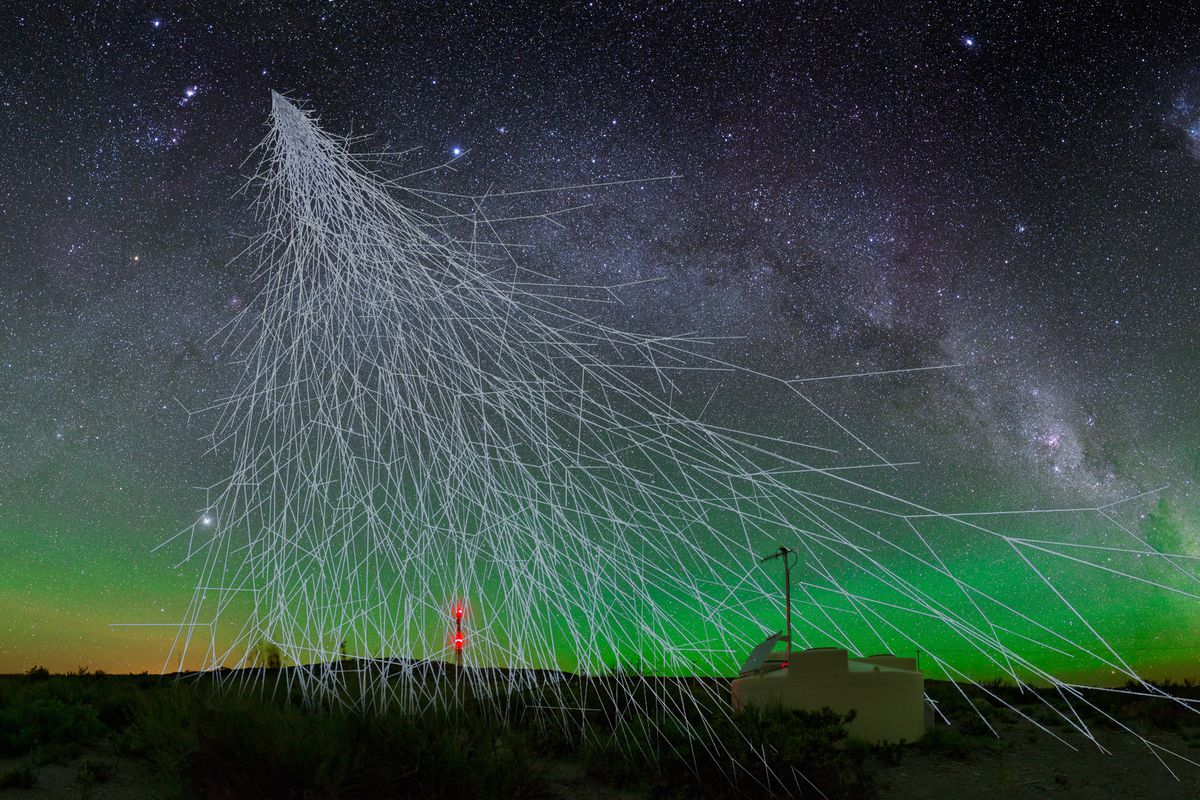
\includegraphics[width=0.9\linewidth]{pierre4HR.0.jpg}
\caption{Sciame prodotto da un raggio cosmico primario. \citep{immagine_cosmici}}
\end{figure}
 I RC sono noti fin dai primi decenni del '900 e la loro fisca è stata studiata approfonditamente nel corso degli anni. Ciononstante, alcuni aspetti non sono stati approfonditi, per cui risulta tutt'ora di grande interesse scientifico effettuare ricerca in questo campo. Le misure di interesse che vogliamo effettuare con il nostro esperimento sono: 
\begin{enumerate}
    \item \textbf{Misura di flusso verticale dei RC carichi in funzione dell'altitudine} - Il flusso verticale di raggi cosmici è atteso dipendere dalla quota: l'interazione adronica dei primari con l'atmosfera (Figura \ref{frammentazione primari}) dipende criticamente dalla densità del mezzo. Stimiamo che il massimo della produzione di secondari avvenga attorno ai 20km. Questa misura è di duplice interesse: correlazione con l'altitudine di formazione delle nuvole, rivelando un possibile ruolo dei RC nella loro formazione (esperimento CLOUD @CERN); stima dei danni da radiazione indotti sull'elettronica, importante per stimare i \textit{single event upset} nella strumentazione di missioni spaziali;
    \begin{figure}
        \centering
        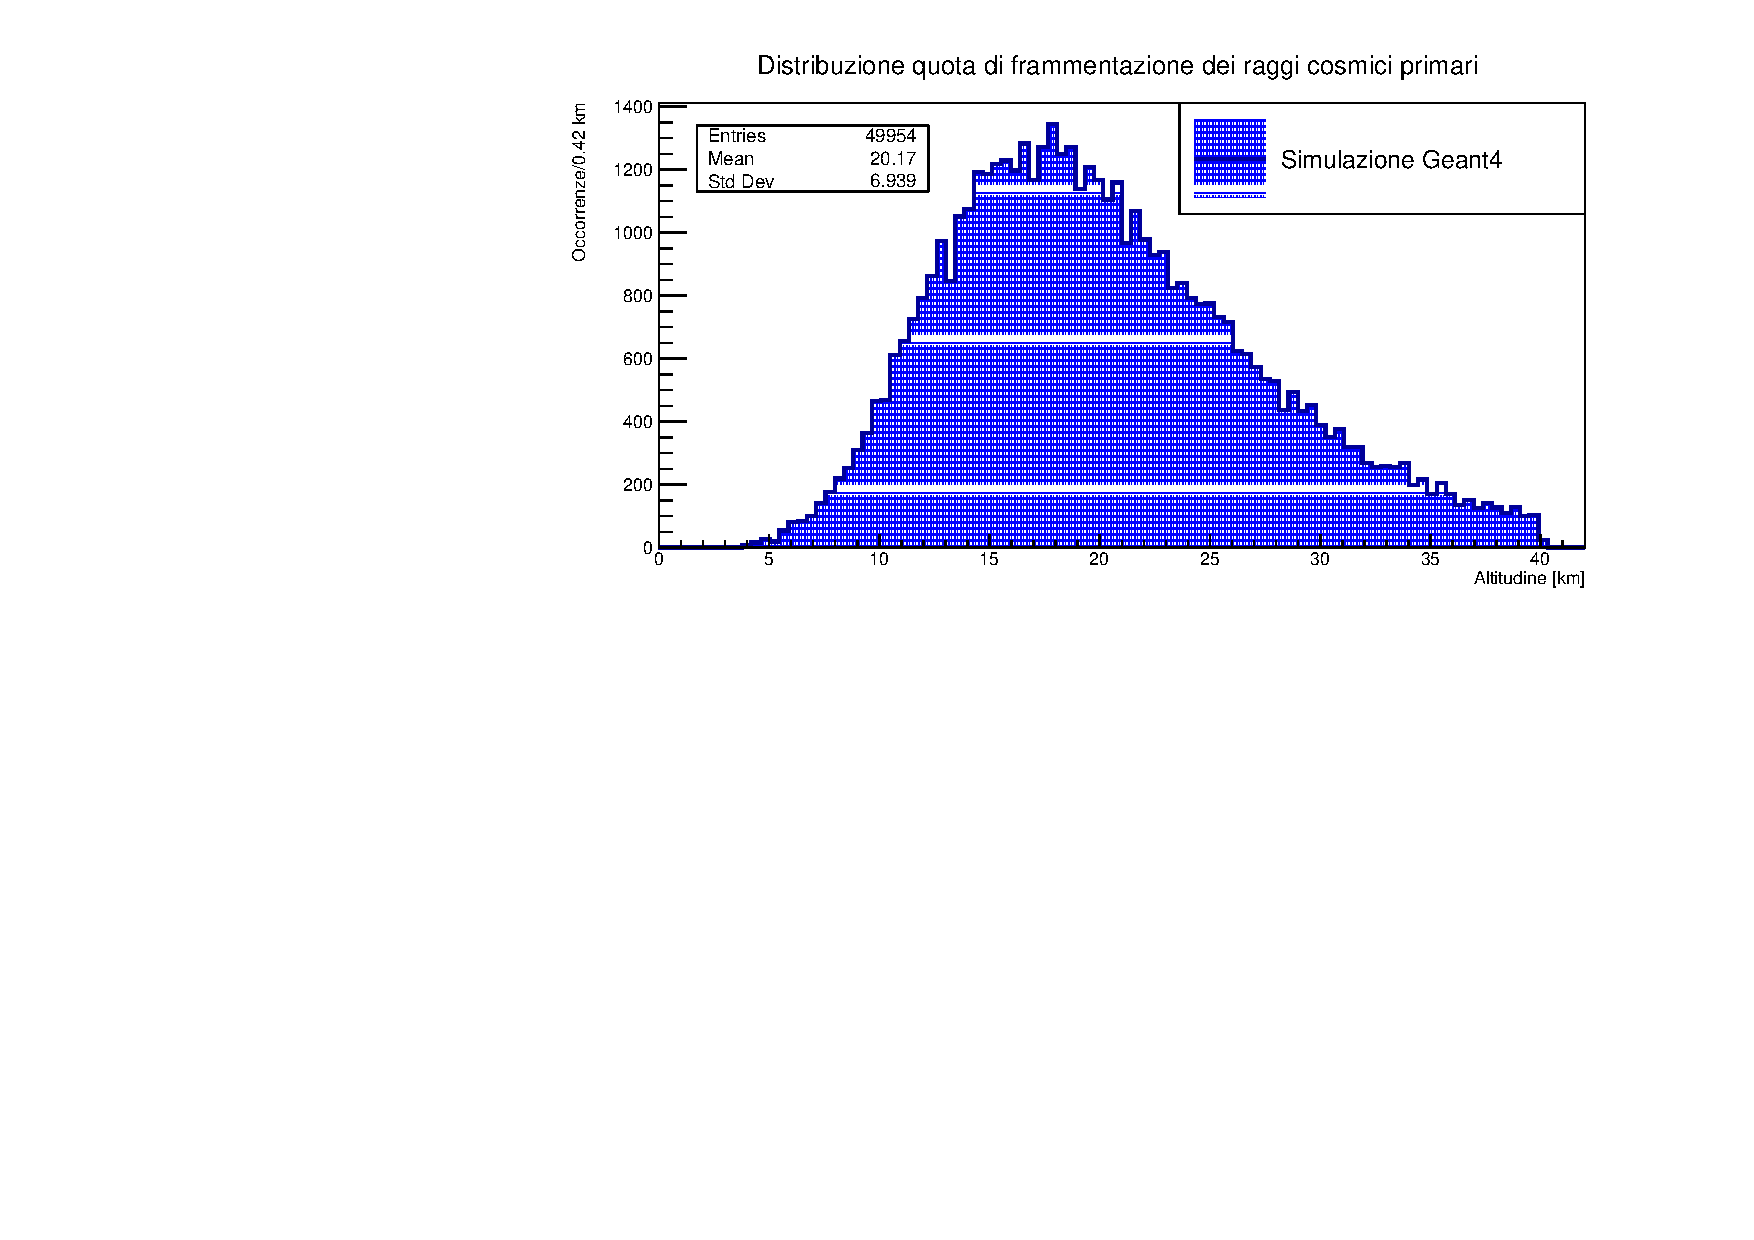
\includegraphics[width=0.9\linewidth]{Frammentazione_verticale.pdf}
        \caption{Simulazione GEANT4 della quota di frammentazione di un fascio di protoni energetici nell'atmosfera.}
        \label{frammentazione primari}
    \end{figure}
    
    \item \textbf{Misura di flusso orizzontale dei RC carichi in funzione dell'altitudine} - Ci si aspetta che la componente orizzontale dei RC sia fortemente soppressa, ma questo dipende dallo spessore trasverso di atmosfera attraversata, dunque dalla quota. Questa misura non è presente in letteratura e può apportare un contributo originale alla comprensione dei RC;
    \item \textbf{Misura del flusso di neutroni termici in funzione dell'altitudine} - I neutroni vengono prodotti in seguito a reazioni di spallazione nucleare tra la componente di raggi cosmici primari ed i nuclei di azoto e ossigeno. Lo spettro energetico risulta piccato per energie di $100\text{ KeV}$, come si osserva dalla Figura \ref{Neutroni}. Attraverso processi di scattering multiplo l'energia cinetica dei neutroni diminuisce, fino ad energie inferiori ad 1 $\text{eV}$. Neutroni con tale range di energie sono definiti termici. A queste energie diventano importanti fenomeni di assorbimento, in particolare si sottolinea il seguente:
\ce{n + ^{14}N -> ^{14}C + p}
, in cui da un nucleo di azoto si forma un particolare isotopo del carbonio. La reazione descritta regola la produzione e abbondanza relativa del carbonio-14 in natura. Dalla misura del flusso di neutroni termici possiamo ricavare il rate di produzione del $^{14}\text{C}$ in funzione della quota (Figura \ref{Carbonio}).
La misura è importante perché l'attività legata al carbonio-14 è uno dei metodi più diffusi di datazioni di reperti organici. 
\begin{figure}
    \centering
    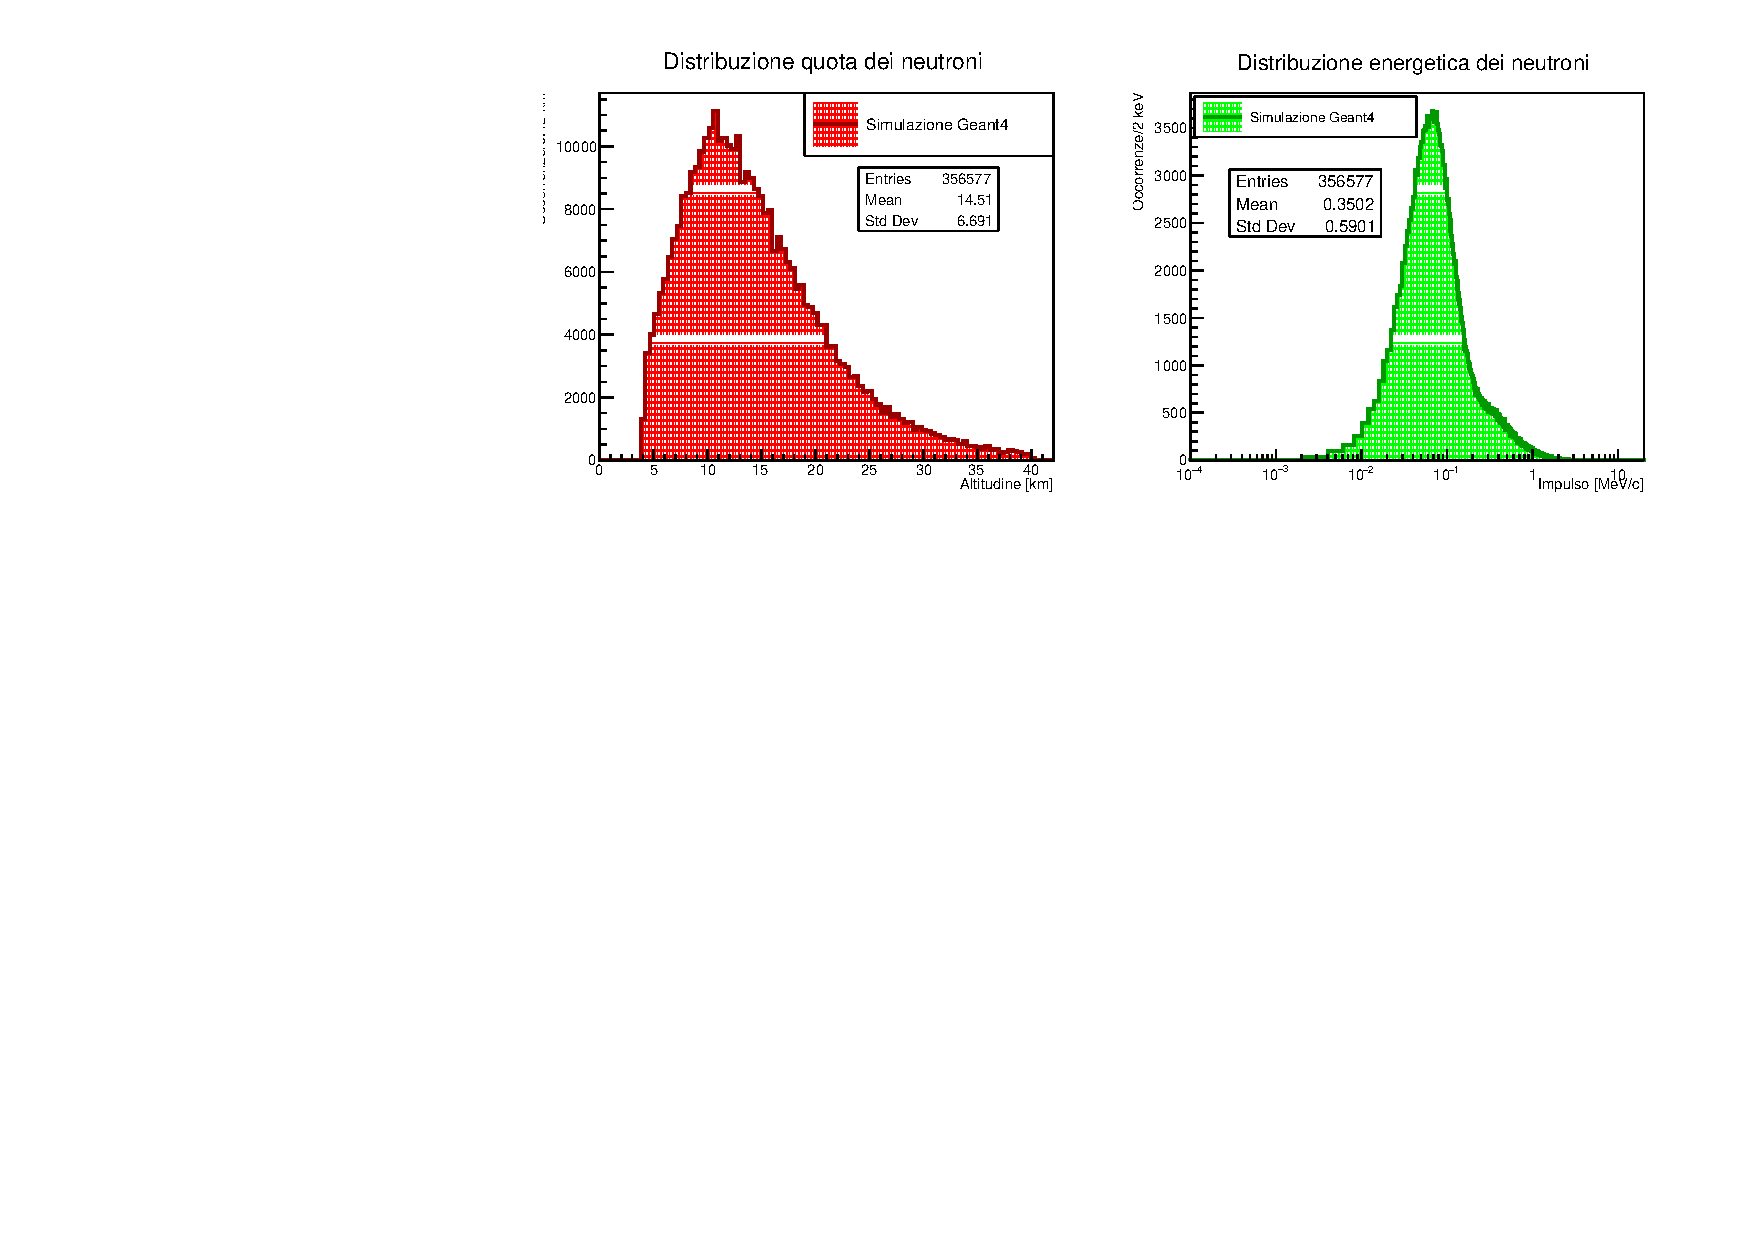
\includegraphics[width=.9\linewidth]{Neutroni.pdf}
    \caption{Simulzione GEANT4 della quota e spettro energetico iniziale dei neutroni prodotti. Si noti come la distribuzione in quota segue quella dei protoni primari (Fig. \ref{frammentazione primari}).}
    \label{Neutroni}
\end{figure}
\begin{figure}
    \centering
    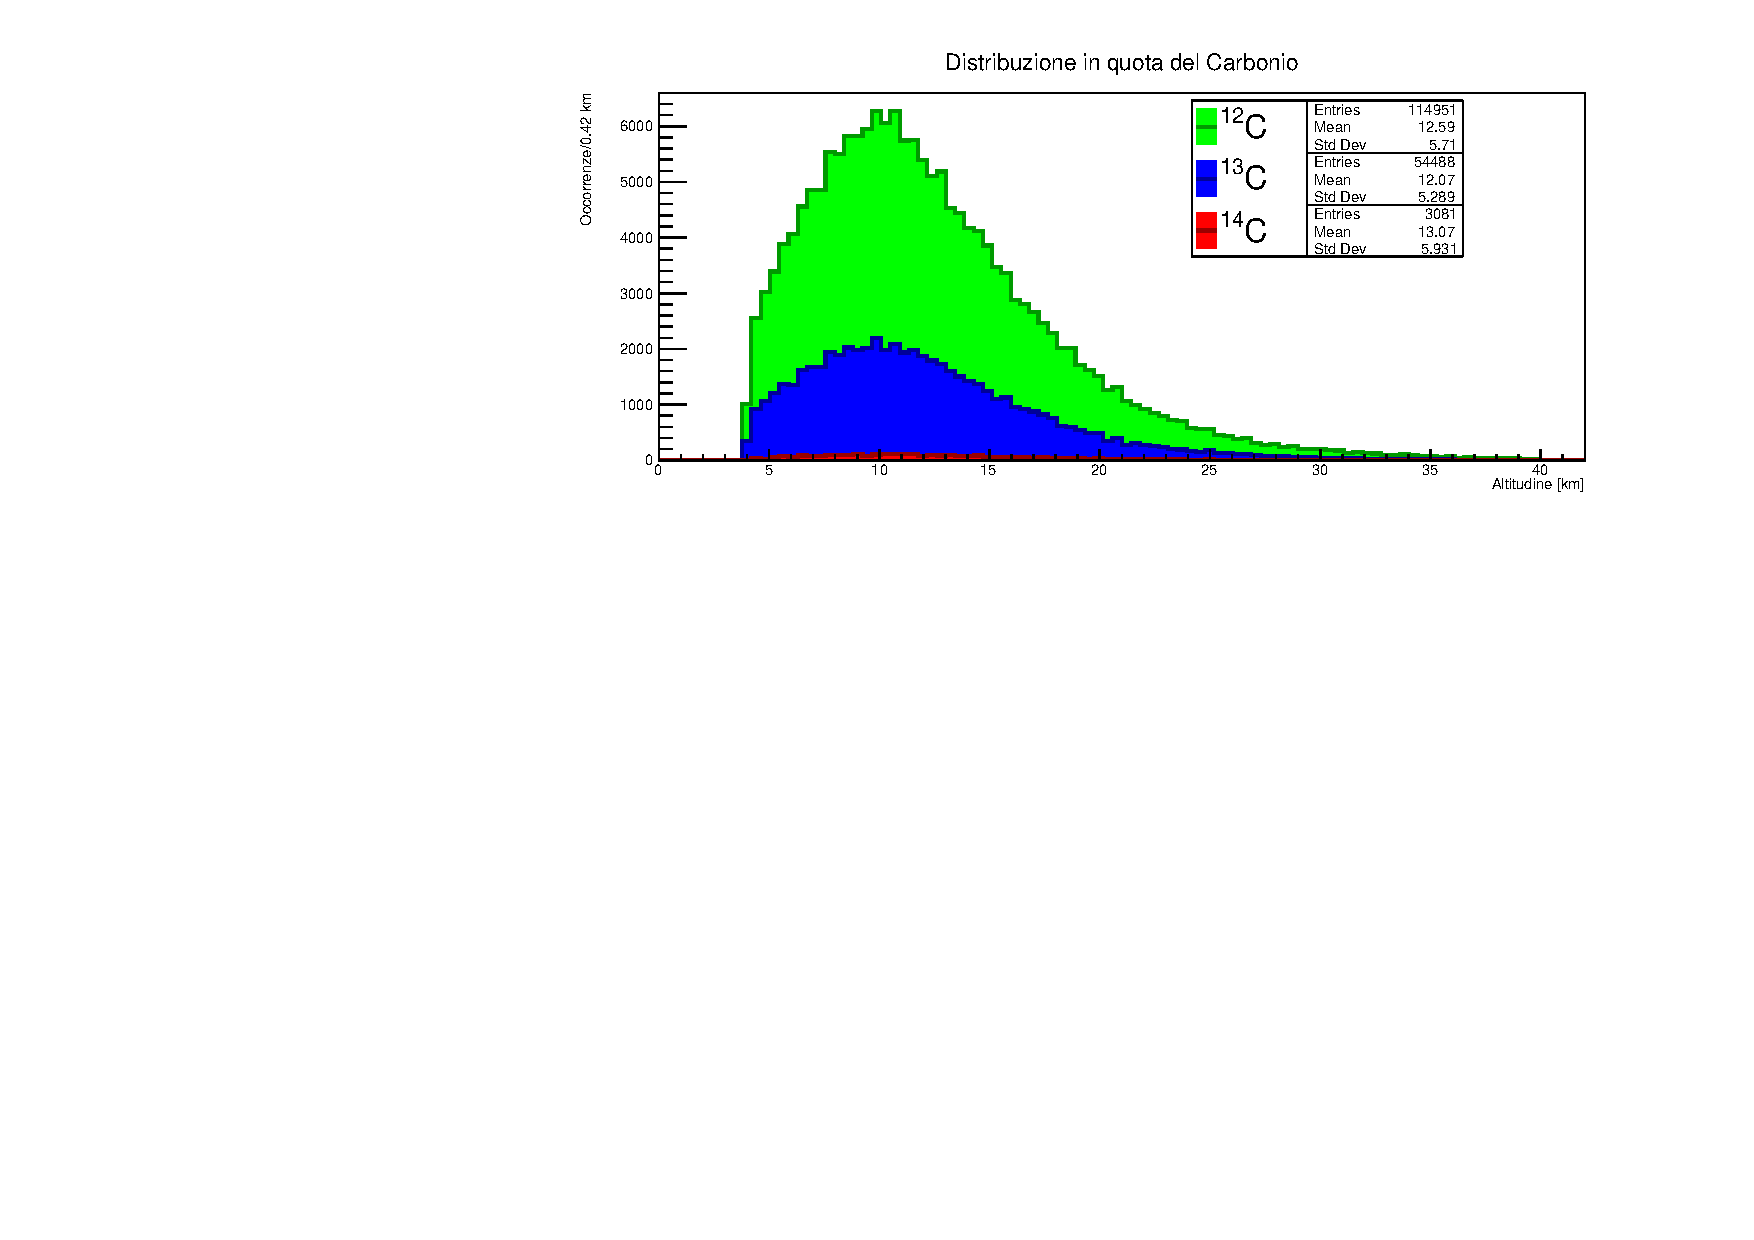
\includegraphics[width=.9\linewidth]{Carbonio_verticale.pdf}
    \caption{Simulazione GEANT4 della distribuzione in quota degli isotopi del C prodotti dai RC primari.}
    \label{Carbonio}
\end{figure}
    \item \textbf{Caratterizzazione del modulo rivelatore \emph{micromegas}} - Prodotto *** DA CHI *** appositamente per il nostro esperimento, ci proponiamo di caratterizzare  la risposta di questo rivelatore in ambienti estremi di temperatura e pressione. Questo lavoro potrebbe essere determinante nella futura applicazione della micromegas a      bordo di satelliti e missioni spaziali. ***** DA COMPLETARE CON ENA ********
\end{enumerate}
\bibliographystyle{plain}
\bibliography{references}


\section{Presentazione del gruppo}

\begin{crewbio}{Adriano Del Vincio}
Laurea triennale in fisica e attualmente iscritto al corso di laurea magistrale in fisica medica. Il mio ruolo all'interno del gruppo è legato all'analisi dati ed ho contribuito a definire la misura proposta del flusso di neutroni in alta atmosfera ed il suo importante legame con la produzione di carbonio 14, impiegato nelle misure di datazione.Inoltre sono stato di supporto a Daniele Passaro nella realizzazione della simulazione dell'interazione di raggi cosmici con l'atmosfera,attraverso l'uso del programma \emph{GEANT4}. 
\end{crewbio}

\begin{crewbio}{Viola Floris}
Laureata in Fisica presso l'Università degli Studi di Perugia. Ho sviluppato una tesi triennale sulla misura dell'energia in Fisica delle Particelle mediante calorimetri, approfondendo l'esperimento NA62 al SPS (Cern). Attenta ai dettagli ed amante delle sfide, mi sono appassionata agli aspetti più sperimentali della fisica delle particelle visitando i tunnel del Cern. Attualmente frequento il Corso di Laurea Magistrale in \emph{Interazioni Fondamentali} all'Università di Pisa, dove, grazie al corso di laboratorio, sto portando avanti misure sui raggi cosmici, sul decadimento del muone e sull'annichilazione del positrone. Do il mio contributo al progetto con l'esperienza acquisita proprio in queste misure.
\end{crewbio}

\begin{crewbio}{Daniele Passaro}
Sono uno studente iscritto al corso di laurea magistrale in Fisica presso l'Università di Pisa, curriculum di  "Interazioni Fondamentali". 
Il mio percorso formativo è incentrato sulla fisica delle particelle, in particolare dando grande attenzione ai metodi sperimentali necessari per l'attività di ricerca in fisica delle alte energie. Riguardo l'attività sperimentale, ho acquisito esperienza seguendo un totale di 6 corsi di laboratorio: 5 durante il corso di laurea triennale in Fisica presso UniSa, incentrati su analisi dati, elettronica digitale e analogica, microelettronica, magnetismo e simulazioni numeriche; uno durante il corso di laurea magistrale, dedicato alla fisica delle interazioni fondamentali ed in particolare sui raggi cosmici.

Nel progetto mi occupo delle simulazioni Monte Carlo, realizzate tramite il toolkit di simulazione avanzata GEANT4 (\textcopyright CERN), e collaboro alla caratterizzazione generale della strumentazione . 
\end{crewbio}

\begin{crewbio}{Domenico Riccardi}
Sono iscritto al corso di laurea magistrale in Fisica presso l'Università di Pisa, curriculum di "Interazioni Fondamentali". I miei interessi sono rivolti, principalmente, alla fisica sperimentale delle alte energie e all'analisi dei dati. L'attività sperimentale svolta nel corso della laurea triennale, frequentando tre laboratori, e in quella magistrale, con il laboratorio d'interazioni fondamentali, mi hanno permesso di approfondire aspetti e problematiche nell'ambito della realizzazione e dell'analisi dei risultati di esperimenti scientifici. La mia passione per la fisica delle alte energie, mi ha portato ad un lavoro di tesi triennale incentrato sullo studio dell'efficienza di ricostruzione dei muoni nel decadimento del mesone $B_c^+$ su simulazioni Monte Carlo prodotte dall'esperimento CMS ad LHC. Nell'esperimento concepito mi occupo dello studio dell'efficienza dell'apparato, che è una variabile fondamentale per le misure di flusso che si vogliono ricavare, e più in generale sulla sua caratterizzazione.
\end{crewbio}

\begin{crewbio}{Marco Riggirello}
Sono uno studente magistrale del dipartimento di Fisica dell'Università di Pisa iscritto al curriculum di \emph{Fisica delle Interazioni Fondamentali}. Per la laurea triennale, conseguita nel 2020, ho presentato una tesi sulla misura della violazione dell'universalità leptonica con l'esperimento CMS in cui ho effettuato un'analisi volta a ottimizzare la precisione della misura di $R(J/\psi)$. Sono molto interessato alle sfide sperimentali della fisica delle alte energie: durante il mio percorso triennale ho seguito numerosi corsi su argomenti di elettronica e analisi dati che sto approfondendo nella prosecuzione magistrale. 

Per il nostro progetto mi sono occupato del \emph{design} dell'apparato e, se sarà effettuato il lancio, contribuir\`o all'analisi dei dati raccolti.
\end{crewbio}

\begin{crewbio}{Antoine Venturini}
Sono uno studente della laurea magistrale in Fisica presso l'Università di Pisa, iscritto al curriculum di Interazioni Fondamentali. Ho coltivato l'interesse per la fisica delle particelle sin dagli anni della triennale, laureandomi (nel 2020) con una tesi sulla misura del decadimento raro del bosone di Higgs in $\mu^+ \mu^-$ di LHC @CERN, e frequentando poi la stessa estate la Summer School tenuta in Giappone dalla collaborazione per l'esperimento Belle 2.  
Insieme ai corsi teorici seguo numerosi corsi dedicati agli aspetti sperimentali della ricerca in fisica delle alte energie, sia all'analisi dati che alla strumentazione per la rivelazione delle particelle.
Ho alle spalle l'esperienza di quattro corsi di laboratorio, dedicati all'analisi dati e all'elettronica analogica e digitale. In particolare, nell'ultimo anno ho condotto esperienze sulla rivelazione di raggi cosmici per mezzo di rivelatori a scintillazione e fototubi. 

Nell'ambito del nostro progetto, mi occupo del sistema per la rivelazioni dei neutroni e dell'analisi dei dati raccolti (se tutto andrà bene). 
\end{crewbio}



\section{Rivelatore di neutroni}
Essendo particelle neutre, i neutroni non possono essere rivelati con \emph{detectors} che sfruttano il principio della ionizzazione, perciò una strumentazione dedicata è necessaria. I rivelatori di neutroni sono basati sulla rivelazione di prodotti secondari (fotoni, particelle cariche) dalle reazioni nucleari indotte dall'urto del neutrone su elementi tipo $^{10}$B o $^6$Li. Questo sistema di rivelazione è efficace solo per i neutroni termici, e proprio per questo è ideale per la misura sul flusso di neutroni che ci proponiamo di svolgere. Entrambi i sistemi che vengono proposti sono basati su una plastica drogata accoppiata ad un rivelatore di fotoni: i costi ed il peso sono simili, ma hanno pregi e difetti che richiedono un approfondimento maggiore per scegliere quale utilizzare nell'esperienza (\emph{che svolgeremo appena il progetto venga approvato}). 

\subsection{Prima proposta}
Un sistema utilizza come rivelatore il dosimetro CT007-T della GammaGuard. Il dosimetro comunica tramite Bluetooth con una applicazione per Android, dove i dati (compresi data e coordinate GPS) vengono conservati. Il salvataggio dei dati su un file .csv viene eseguito attraverso comandi manuali alla fine dell'acquisizione, perciò questo sistema prevede la necessità di un cellulare che rimanga funzionante in volo e dopo l'atterraggio. Un cellulare che soddisfa le richieste è il Blackview BV4900 ProRugged (operatività garantita a temperature nel range [-55, +70] °C). 

\textbf{Pregi}: 1) un rivelatore pronto all'uso e con una interfaccia semplice e dai risultati garantiti; 2) il peso complessivo (400 g); 3) l'alimentazione autonoma (due pile AA per il dosimetro, la batteria per il cellulare); 4) il cellulare supporta la ricarica inversa, perciò potrebbe essere utilizzato come power bank (\emph{da valutare in laboratorio}). 

\textbf{Difetti}: 1) Impossibilità di salvare i dati automaticamente. 

\subsection{Seconda proposta}
La seconda proposta prevede di utilizzare un rivelatore della ditta Scionix che accoppia un rivelatore di fotoni a semiconduttore a un materiale drogato con $^6$Li. Il sistema viene letto da un circuito elettronico simile a quello già montato per il rivelatore di particelle cariche (e sfrutta parte di quella elettronica).
\textbf{Pregi}: 1) Il dispositivo è realizzato dalla ditta Scionix su misura per il nostro scopo, e sfrutta il \emph{know-how} dell'INFN per realizzare un sistema affidabile, perciò il recupero dei dati è garantito; 2) peso ($\sim$ 400 g).
\textbf{Difetti}: 1)  \`E necessario montare un ulteriore power bank per alimentare il rivelatore; 2) l'assemblamento del sistema è più complesso di quello della prima proposta. 





\end{document}

